\chapter{Evaluation}



explain the benchmarking setup and reason why certain setup choices were made

incorporate paper for statistical analysis which explains number of rounds etc

explain the benchmark problems and their specific attributes

show here that the approach in total is feasable

show the optimizations through better scheduling

discuss inexplicable results

\section{Local Distribution}

\begin{figure}[H]
	
	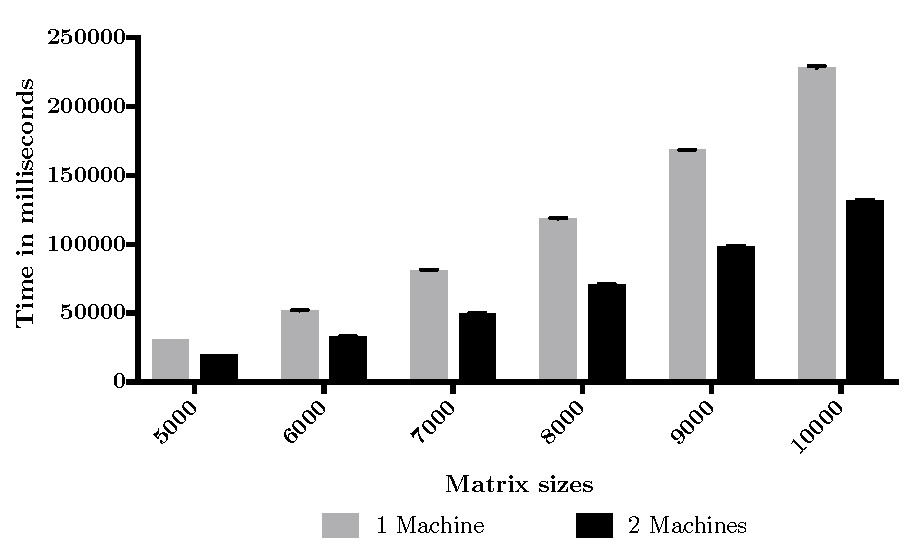
\includegraphics[width=1.0\textwidth]{images/sharded_matrix_multi.pdf}
	\centering
	\caption{Parallel Matrix Multiplication}
	\label{img:parallel_matrix}
\end{figure}


\begin{figure}[H]
	
	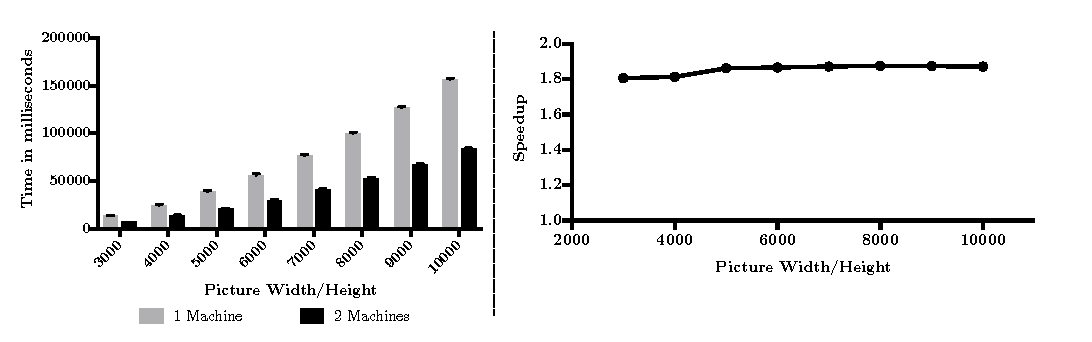
\includegraphics[width=1.0\textwidth]{images/sharded_mandelbrot.pdf}
	\centering
	\caption{Parallel Mandelbrot}
	\label{img:parallel_mandelbrot}
\end{figure}

\begin{table}[!htb]
	\centering
	\begin{adjustbox}{width=0.95\textwidth}
		\small
		\begin{tabular}{l | l | l | l}
			~							& \textbf{Size}		& \textbf{Iterations}	& \textbf{Kernels per Iteration} \\
			\hline
			\textbf{Matrix Multiplication 1 (MM1)} 	& 8000x8000  								& 1 	& 5 \\
			\textbf{Matrix Multiplication 2 (MM2)}     & 6000x6000  								& 1		& 5 \\
			\textbf{Mandelbrot 1 (MB1)}     			& 1000x1000 (1000000 iterations per point) 	& 1		& 5 \\
			\textbf{Mandelbrot 2 (MB2)}     			& 2000x2000 (600000 iterations per point)  	& 1		& 5 \\
			\textbf{K-means (KM)}          			& 6000000 objects and 200 clusters  		& 10	& 1 \\
			\textbf{N-body (NB)}    		 			& 64000 objects  							& 10	& 1 \\		
		\end{tabular}
	\end{adjustbox}
	
	\caption{Benchmark Job Setup}
	\label{table:benchmark_job_setup}
\end{table}

\begin{figure}[H]
	
	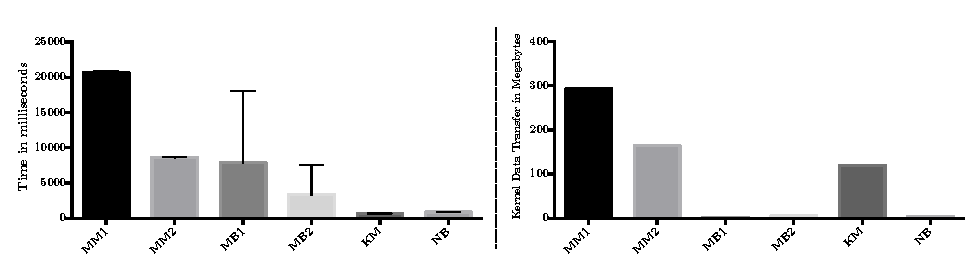
\includegraphics[width=1.0\textwidth]{images/benchmark_kernel_data_transfers.pdf}
	\centering
	\caption{Average Kernel Runtimes and Data Transfer Sizes}
	\label{img:benchmark_kernel_attributes}
\end{figure}

\section{Hybrid Distribution}



benchmark selection
scheduler selection
benchmark setup: first submit all jobs, then start execution at once
why do iterative tasks have less kernels
mention utilized aws region